
%!TEX option = --shell-escape

\documentclass[9pt, xcolor={svgnames, x11names},professionalfonts]{beamer}

 \definecolor{saitPurple}{RGB}{112,40,119}
 \definecolor{statsMaroon}{rgb}{0.55, 0, 0}
 \definecolor{saitMaroon}{rgb}{0.55, 0, 0}
 \definecolor{statsRed}{RGB}{224,38,37}
 \definecolor{saitRed}{RGB}{224,38,37}
 \definecolor{saitBlue}{rgb}{0, 0.59, 0.85}
 \definecolor{statsBlue}{rgb}{0, 0.59, 0.85}
 \definecolor{statsDeepBlue}{RGB}{0, 99, 167}
 \definecolor{saitDeepBlue}{RGB}{0, 99, 167}
 \definecolor{saitDeepBlue}{RGB}{0, 99, 167}
 \definecolor{LightGrey}{RGB}{200,200,200}
%  \definecolor{boxBG}{RGB}{236, 227, 227}
%  \definecolor{boxBG}{RGB}{242, 233, 223}
\usepackage{xcolor}
\usepackage{cancel}
\usepackage{bm}
\usepackage{graphicx}
\usepackage[x11names, svgnames]{xcolor} % for colors in handouts, auto loaded in Beamer?
\usepackage{tikz}
\usetikzlibrary{arrows.meta, math, calc, shadows}
\usetikzlibrary{decorations.markings, decorations.fractals, decorations.text} % for chain, etc.
\usetikzlibrary{intersections}
\usepackage{pgfmath}
\usepackage{ifthen}
\usepgfmodule{oo}
\usepgflibrary{shadings}
% \usetikzlibrary{decorations.shapes}
\usepackage[many]{tcolorbox}
\usepackage[absolute,overlay,showboxes]{textpos}
% \usepackage{textpos}
% \textblockorigin{0.0cm}{0.0cm}  %start all at upper left corner
\TPshowboxesfalse

\newcommand\lb{\linebreak}
\newcommand\Ra{\Rightarrow}
\newcommand\cd{\!\cdot\!}
\newcommand\x{\!\times\!}
\newcommand\pars{\par\smallskip}
\newcommand\parm{\par\medskip}
\newcommand\parb{\par\bigskip}
\renewcommand{\deg}{^\circ}

% counter for resuming enumerated list numbers
\newcounter{resumeenumi}
\newcommand{\suspend}{\setcounter{resumeenumi}{\theenumi}}
\newcommand{\resume}{\setcounter{enumi}{\theresumeenumi}}



% https://tex.stackexchange.com/questions/33703/extract-x-y-coordinate-of-an-arbitrary-point-in-tikz
\makeatletter
\providecommand{\gettikzxy}[3]{%
	\tikz@scan@one@point\pgfutil@firstofone#1\relax
	\edef#2{\the\pgf@x}%
	\edef#3{\the\pgf@y}%
}
\makeatother

\makeatletter
\newcommand{\verbatimfont}[1]{\def\verbatim@font{#1}}%
\makeatother

%%%%%%%%%%%%%%%%%%%%%%%%%%%%%%%%%%%%%%%%%%%%%%%%%%%%%%%%%%%%%%%%%%%%%%%%%%%%%%%%


\newcommand{\tb}[4][0.8]{
	\begin{textblock*}{#1}(#2, #3)
		% \raggedright
		#4
	\end{textblock*}
}

\newtcolorbox{statsbox}[2][] { 
  colback=white,
  colbacktitle=structure,
  colframe=structure,
  coltitle=white,  
  top=0.25cm,
	bottom=0.125cm,
	left=0mm,
	right=0mm,
  % fonttitle=\itshape\rmfamily,
  halign=flush left, 
  enhanced,
  drop fuzzy shadow,
  attach boxed title to top left={xshift=3.5mm, yshift=-2mm},
  title={#2}, #1}
\newtcolorbox{redbox}{colback=white, colframe=structure, enhanced, drop fuzzy shadow}
\newtcolorbox{titledbox}[1]{colback=white,colframe=structure,title={#1}}
\newtcbox{\tcb}[1][]{colback=white,boxsep=0pt,top=5pt,bottom=5pt,left=5pt,
		right=5pt, colframe=structure,  enhanced, drop fuzzy shadow, #1}
% tcb title
\newtcbox{\tcbt}[2][]{colback=white,boxsep=0pt,top=5pt,bottom=5pt,left=5pt,
		right=5pt, colframe=structure, enhanced, drop fuzzy shadow,  title={#2}, #1}
% tcb left title
\newtcbox{\tcbtl}[2][]{ colback=white,
  colbacktitle=structure,
  colframe=structure,
  coltitle=white,  
  top=0.25cm,
	bottom=0.125cm,
	left=0mm,
	right=0mm,
  % fonttitle=\bfseries,
  halign=flush left, 
  enhanced,
  drop fuzzy shadow,
  attach boxed title to top left={xshift=3.5mm, yshift=-2mm}, 
	title={#2}, #1}

\newtcbtheorem{myexam}{Example}%
{
	enhanced,
	colback=white,
	colframe=structure,
	% fonttitle=\bfseries,
	fonttitle=\itshape\rmfamily,
	drop fuzzy shadow,
	%description font=\mdseries\itshape,
	attach boxed title to top left={yshift=-2mm, xshift=5mm},
	colbacktitle=structure
	}{exam}% then \pageref{exer:theoexample} references the theo

% \newcommand{\myexample}[2][red]{
% 	% \tcb\tcbset{theostyle/.style={colframe=red,colbacktitle=yellow}}
% 	\begin{myexam}{}{}
% 		#2
% 	\end{myexam}
% 	% \tcbset{colframe=structure,colbacktitle=structure}
% }

\newtcbtheorem{myexer}{Exercise}%
{
	enhanced,
	colback=white,
	colframe=structure,
	% fonttitle=\bfseries,
	drop fuzzy shadow,
	fonttitle=\itshape\rmfamily,
	% description font=\mdseries\itshape,
	attach boxed title to top left={yshift=-2mm, xshift=5mm},
	colbacktitle=structure
	}{exer}



\newcommand{\mini}[2][0.8]{
	\begin{minipage}[c]{#1\columnwidth}
		\raggedright
		#2
	\end{minipage}
}
\newcommand{\minit}[2][0.8]{
	\begin{minipage}[t]{#1\columnwidth}
		% \raggedright
		#2
	\end{minipage}
}

% centered minipage with text \raggedright
%\cmini[width]{content}
\newcommand{\cmini}[2][0.8]{
	\begin{center}
		\begin{minipage}{#1\columnwidth}
			\raggedright
			#2
		\end{minipage}
	\end{center}
}



\newcommand{\fig}[2][1]{% scaled graphic
	\includegraphics[scale=#1]{#2}
}

% centred framed colored box black border
%\cbox[width]{content}
\newcommand{\cbox}[2][1]{% framed centered color box
	\setlength\fboxsep{5mm}
	\setlength\fboxrule{.2 mm}
	\begin{center}
		\fcolorbox{black}{white}{
			\vspace{-0.5cm}
			\begin{minipage}{#1\columnwidth}
				\raggedright
				#2
			\end{minipage}
		}
	\end{center}
	\setlength\fboxsep{0cm}
}

\newcommand{\cfig}[2][1]{% centred, scaled graphic
	\begin{center}
		\includegraphics[scale=#1]{#2}
	\end{center}
}






%\Member{startpt}{endpt}{outer fill color}{inner fill color}{stroke}{height}{radius}{linewidth}
\providecommand{\Member}[8]{
  % name the points
  \coordinate(start) at (#1);
  \coordinate(end) at (#2);
  \edef\ofill{#3}%
  \edef\ifill{#4}%
  \edef\stroke{#5}%
  \edef\height{#6} % cm
  \edef\radius{#7} % cm
  \edef\linewidth{#8} % mm

  \coordinate(delta) at ($ (end)-(start) $);
  \gettikzxy{(delta)}{\dx}{\dy}
  \gettikzxy{(start)}{\sx}{\sy}
  \pgfmathparse{veclen(\dx, \dy)} \let\length\pgfmathresult

  \pgfmathparse{\dx==0}%
  % \ifnum low-level TeX for integers
  \ifnum\pgfmathresult=1 % \dx == 0
    \pgfmathsetmacro{\rot}{\dy > 0 ? 90 : -90}
  \else
    \pgfmathsetmacro{\rot}{\dx > 0 ? atan(\dy / \dx) : 180 + atan(\dy / \dx)}
  \fi

  
   
  \shadedraw[transform canvas = { rotate around = {\rot:(\sx,\sy)}}, line width = \linewidth, rounded corners = \radius mm, top color = \ofill, bottom color = \ofill, middle color = \ifill, draw = \stroke] ($ (start)+(-0.5*\height, 0.5*\height) $) -- ++(\height cm +\length pt, 0 ) -- ++(0, -\height) -- ++ (-\height cm -\length pt, 0) -- cycle;


  \shadedraw[ball color = \ofill!50!\ifill, draw = \stroke] (start) circle (\height/8);
  \shadedraw[ball color = \ofill!50!\ifill, draw = \stroke] (end) circle (\height/8);
  %  \pgfresetboundingbox

  
  


}


\newcommand{\PC}[6][0]{%
  \edef\lrotate{#1}%
  \edef\lpin{#2}%
  \edef\lfill{#3}%
  \edef\ldraw{#4}%
  \edef\lscale{#5}%
  \edef\lwidth{#6}% mm
  \edef\h{1}%
  \edef\r{0.3}%
  \begin{scope}[scale=\lscale, rotate=\lrotate]
	\filldraw[draw=\ldraw, fill=\lfill, line width=\lwidth mm] ($ (\lpin) + (0.201*\h+1.0353*\r ,-0.75*\h) $) -- ++(105: 0.77646*\h+0.26795*\r) arc (15:165:\r) -- ++(-105:0.77646*\h+0.26795*\r) -- cycle;

	\shadedraw[ball color=\lfill, draw=\ldraw, line width = \lwidth mm] (\lpin) circle (1.5mm);

	\filldraw[rounded corners=\lscale pt, draw=\ldraw, fill=\lfill, line width=\lwidth mm] ($ (\lpin) - (1,1) $) rectangle +(2,0.25);
  \end{scope}%
}




\usepackage{mathtools}
\usepackage{xcolor}
\usefonttheme[onlymath]{serif} 
\usepackage{mathpazo}
\usepackage{bm}
\usepackage{cancel}
\usepackage[many]{tcolorbox}
% \tcbset{fonttitle=\itshape\rmfamily\bfseries}
\tcbset{fonttitle=\itshape\rmfamily}
\usepackage{tikz}
\usetikzlibrary{arrows.meta, math, calc, shadows}

\usepackage{pgfplots}
\pgfplotsset{compat=1.18}

\usefonttheme{structureitalicserif} %make titles fancy ;-)
\usefonttheme[onlymath]{serif}

\usecolortheme[named=statsMaroon]{structure}
\setbeamertemplate{navigation symbols}{} % remove navigation symbols
\setbeamertemplate{headline}{\vspace{0.125cm}}
\setbeamertemplate{footline}{ \hfill \insertshorttitle\qquad \insertsection \qquad \insertframenumber/\inserttotalframenumber\quad{ }\vspace{0.125cm}}
\setbeamertemplate{items}[default]
\setbeamertemplate{blocks}[shadow=true]

\setbeamercolor{title}{bg=statsMaroon, fg=Azure}
\setbeamercolor{frametitle}{fg=white, bg=statsMaroon}
\setbeamercolor{background canvas}{bg=Gainsboro!50}
\setbeamercolor{block title}{bg=statsMaroon, fg=white}
\setbeamercolor{block body}{bg=white, fg=black}

\setlength{\parskip}{\medskipamount}
\setlength{\parindent}{0pt}

\def\scale{1}
\newcounter{myexercisecounter}

% Title page details: 
\title[Force Vectors]{\Huge 02 Force Vectors}
\subtitle[Engineering Statics]{\Large\textcolor{white}{Engineering Statics}}
\author{}
\date{\small Updated on: \today}

% \raggedright

%%%%%%%%%%%%%%%%%%%%%%%%%%%%%%%%%%%%%%%%%%%%%%%%%%%%%%%%%%%%%%%%%%%%%%%%%%%%%%%%

\begin{document}

%%%%%%%%%%%%%%%%%%%%%%%%%%%%%%%%%%%%%%%%%%%%%%%%%%%%%%%%%%%%%%%%%%%%%%%%%%%%%%%%
\newtcolorbox{statsbox}[2][] {  
  % colback=Ivory3!50,
  colback=white,
  colbacktitle=structure,
  colframe=structure,
  coltitle=white,  
  top=0.25cm,
	bottom=0.125cm,
	left=0mm,
	right=0mm,
  % fonttitle=\itshape\rmfamily,
  halign=flush left, 
  enhanced,
  drop fuzzy shadow,
  attach boxed title to top left={xshift=3.5mm, yshift=-2mm},
  title={#2}, #1}
\newtcolorbox{redbox}{colback=white, colframe=structure, enhanced, drop fuzzy shadow}
\newtcolorbox{titledbox}[1]{colback=white,colframe=structure,title={#1}}
\newtcbox{\tcb}[1][]{colback=white,boxsep=0pt,top=5pt,bottom=5pt,left=5pt,
		right=5pt, colframe=structure,  enhanced, drop fuzzy shadow, #1}
% tcb title
\newtcbox{\tcbt}[2][]{colback=white,boxsep=0pt,top=5pt,bottom=5pt,left=5pt,
		right=5pt, colframe=structure, enhanced, drop fuzzy shadow,  title={#2}, #1}
% tcb left title
\newtcbox{\tcbtl}[2][]{ colback=white,
  colbacktitle=structure,
  colframe=structure,
  coltitle=white,  
  top=0.25cm,
	bottom=0.125cm,
	left=0mm,
	right=0mm,
  % fonttitle=\bfseries,
  halign=flush left, 
  enhanced,
  drop fuzzy shadow,
  attach boxed title to top left={xshift=3.5mm, yshift=-2mm}, 
	title={#2}, #1}

%%%%%%%%%%%%%%%%%%%%%%%%%%%%%%%%%%%%%%%%%%%%%%%%%%%%%%%%%%%%%%%%%%%%%%%%%%%%%%%%

\begin{frame}[plain]    %don't need footer on titlepage
	\titlepage
\end{frame}

%%%%%%%%%%%%%%%%%%%%%%%%%%%%%%%%%%%%%%%%%%%%%%%%%%%%%%%%%%%%%%%%%%%%%%%%%%%%%%%%


%%%%%%%%%%%%%%%%%%%%%%%%%%%%%%%%%%%%%%%%%%%%%%%%%%%%%%%%%%%%%%%%%%%%%%%%%%%%%%%%

\begin{frame}{Scalars versus Vectors }
	% centered minipage with text raggedright
	%cmini[width]{content}
	\cmini[0.8]{
		\begin{redbox}
		\begin{itemize}
			\item Physical quantities in this course are measured using either {\bf
				scalars} or {\bf vectors}.\parm
			\item A scalar quantity can be fully specified by its {\bf magnitude}
			      (or size) and units alone. \pars Examples are temperature, speed, mass, time,
			      length, volume, density and energy.\parm
			\item A vector quantity requires both magnitude {\bf and direction} -
			      in addition to units - to be fully specified. \pars Examples are displacement,
			      velocity, force and momentum.\parm
			\item 110 km/h is a speed. 110 km/h in a north-easterly direction is a vector.\parm
			\item The vector quantity that is of most interest to us is {\bf
			force}.
		\end{itemize}
	\end{redbox}
	}
\end{frame}

%%%%%%%%%%%%%%%%%%%%%%%%%%%%%%%%%%%%%%%%%%%%%%%%%%%%%%%%%%%%%%%%%%%%%%%%%%%%%%%%

\begin{frame}{Graphical Vector Representation}
	\cmini[1]{
		\begin{redbox}
			\begin{itemize}
				\item To represent a vector on a diagram, we draw a directed line
							segment -- a line with an arrow tip.
				\item The length of the line segment is proportional to the magnitude of the
							vector.
				\item The direction of the line segment shows the direction of the vector.
				\item The arrow head gives the sense of that direction (up and rightwards in this case).
			\end{itemize}
		\end{redbox}
	}
	\mini[0.35]{
		\tcb{
			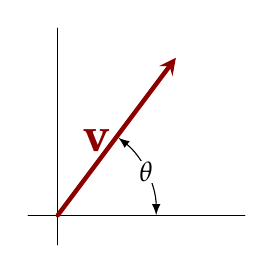
\begin{tikzpicture}[scale = 0.5, style={line cap = round}]
  % \filldraw [thick, white, draw=saitMaroon, drop shadow={opacity=0.25}] (-1, -1) rectangle (5,5);
  \draw (-0.75,0) -- (4.75,0);
  \draw (0, -0.75) -- (0, 4.75);
  \draw[ultra thick, saitMaroon, ->, >=stealth] (0, 0) -- (3, 4) node [xshift=-1cm, yshift=-1.05cm] {\LARGE ${\bm{\mathrm{ v }}}$};
  \only<2>{
    \draw[latex-latex] (2.5, 0) arc (0:52:2.5cm)  node[midway, fill=white, inner sep=0.1mm]{$\theta$};
  }
\end{tikzpicture}

		}
	}
	\uncover<2->{
		\hfill	
		\mini[0.6]{	
			\begin{statsbox}[left=0mm]{}
				\begin{itemize}
					\item $\theta$ indicates the direction of the line of action of the vector
								${\bm{\mathrm{ v }}}$  relative to some reference. \lb(I.e., the horizontal axis in this case.)
					
				\end{itemize}
			\end{statsbox}
		}
	}
\end{frame}

%%%%%%%%%%%%%%%%%%%%%%%%%%%%%%%%%%%%%%%%%%%%%%%%%%%%%%%%%%%%%%%%%%%%%%%%%%%%%%%%

\begin{frame}{Multiplication of a vector by a scalar}
	
	\cmini[0.8]{
		\begin{statsbox}[left=5mm, right=5mm]{}
			Multiplication of a vector by a scalar affects the magnitude and, if the scalar is negative, the sense of the direction of the vector.
			\parb	
			\centering
			% !TEX root = ../../statikz/statikz.tex

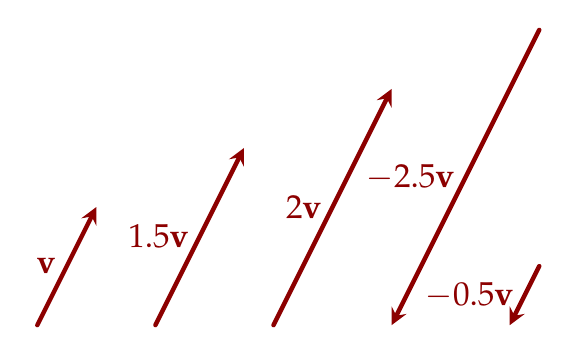
\begin{tikzpicture}[scale = 0.75, style={line cap = round}]

  % \filldraw [white, draw=saitMaroon, thick, drop shadow={opacity=0.25}] (-0.5, -1.5) rectangle (10,4.5);
  \draw[ultra thick, saitMaroon, ->, >=stealth] (0, -1) -- (1, 1) node [xshift=-0.375cm, yshift=-0.75cm, left] {\large ${\bm{\mathrm{ v }}}$};
  \draw[ultra thick, saitMaroon, ->, >=stealth] (2, -1) -- (3.5, 2) node [xshift=-0.5625cm, yshift=-1.125cm, left] {\large ${1.5 \bm{\mathrm{ v }}}$};
  \draw[ultra thick, saitMaroon, ->, >=stealth] (4, -1) -- (6, 3) node [xshift=-0.75cm, yshift=-1.5cm, left] {\large ${2 \bm{\mathrm{ v }}}$};
  \draw[ultra thick, saitMaroon, <-, >=stealth] (6, -1) -- (8.5, 4) node [xshift=-0.9375cm, yshift=-1.875cm, left] {\large ${-2.5 \bm{\mathrm{ v }}}$};
  \draw[ultra thick, saitMaroon, <-, >=stealth] (8, -1) -- (8.5, 0) node [xshift=-.1875cm, yshift=-.375cm, left] {\large ${-0.5 \bm{\mathrm{ v }}}$};

\end{tikzpicture}

		\end{statsbox}
	}
\end{frame}

%%%%%%%%%%%%%%%%%%%%%%%%%%%%%%%%%%%%%%%%%%%%%%%%%%%%%%%%%%%%%%%%%%%%%%%%%%%%%%%%

\begin{frame}{Addition of Vectors}
	% centered minipage with text raggedright
	%cmini[width]{content}
	\cmini[0.8]{

		\mini[0.5]{
			Consider two vectors, $\bm{\mathrm{ A }}$ and $\bm{\mathrm{ B }}$:
		}
		\hfill
		\mini[0.45]{
			\centering
			% !TEX root = ../../statikz/statikz.tex

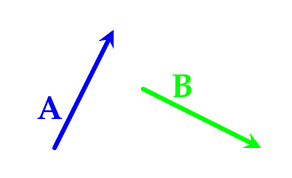
\begin{tikzpicture}[scale =0.75, style={line cap = round}]
  % \filldraw [white, draw=saitMaroon, thick, drop shadow={opacity=0.25}] (0.5, 0.5) rectangle (5,3.5);
  \draw[ultra thick, blue, ->, >=stealth] (1, 1) -- (2, 3) node [xshift=-0.5cm, yshift=-1cm, left] {\large ${\bm{\mathrm{ A }}} $};
  \draw[ultra thick, green, ->, >=stealth] (2.5, 2) -- (4.5, 1) node [xshift=-1cm, yshift=0.5cm, above] {\large ${\bm{\mathrm{ B }}}$};
\end{tikzpicture}

		}
		\parm\pause
		\mini[0.5]{
			To add vectors  $\bm{\mathrm{ A }}$ and  $\bm{\mathrm{ B }}$, written $\bm{\mathrm{ A+B }}$, place the tail of $\bm{\mathrm{ B }}$ at the tip of~$\bm{\mathrm{ A }}$.
		}
		\hfill
		\mini[0.45]{
			\centering
			% !TEX root = ../../statikz/statikz.tex

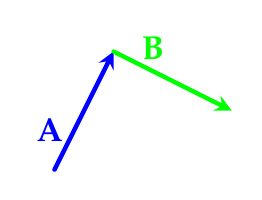
\begin{tikzpicture}[scale =0.75, style={line cap = round}]
  % \filldraw [white, draw=saitMaroon, thick, drop shadow={opacity=0.25}] (0.5, 0.5) rectangle (5,3.5);
  \draw[ultra thick, blue, ->, >=stealth] (1, 1) -- (2, 3) node [xshift=-0.5cm, yshift=-1cm, left] {\large ${\bm{\mathrm{ A }}}$};
  \draw[ultra thick, green, ->, >=stealth] (2, 3) -- (4, 2) node [xshift=-1cm, yshift=0.5cm, above] {\large ${\bm{\mathrm{ B }}}$};
\end{tikzpicture}

		}
		\parm\pause
		\mini[0.5]{
			The sum, $\bm{ A+B}$, is obtained by drawing a vector ${\bm R}$ from the tail of $\bm{\mathrm{ A }}$ to the tip of $\bm{\mathrm{ B }}$.
			\[ \bm{\mathrm{A+B=R}} \]
		}
		\hfill
		\mini[0.45]{
			\centering
			% !TEX root = ../../statikz/statikz.tex

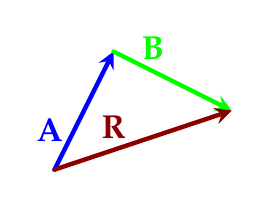
\begin{tikzpicture}[scale =0.75, style={line cap = round}]
  % \filldraw [white, draw=saitMaroon, thick, drop shadow={opacity=0.25}] (0.5, 0.5) rectangle (4.5,3.5);
  \draw[ultra thick, blue, ->, >=stealth] (1, 1) -- (2, 3) node [xshift=-0.5cm, yshift=-1cm, left] {\large ${\bm{\mathrm{ A }}}$};
  \draw[ultra thick, green, ->, >=stealth] (2, 3) -- (4, 2) node [xshift=-1cm, yshift=0.5cm, above] {\large ${\bm{\mathrm{ B }}}$};
  \draw[ultra thick, saitMaroon, ->, >=stealth] (1, 1) -- (4, 2) node [xshift=-1.5cm, yshift=-0.5cm, above] {\large ${\bm{\mathrm{ R }}}$};
\end{tikzpicture}

		}
		\par\pause
		% centered minipage with text raggedright
		%cmini[width]{content}
		\cmini[0.9]{
			{\bf Note that the sum of two vectors is itself a vector.}
		}

	}
\end{frame}

%%%%%%%%%%%%%%%%%%%%%%%%%%%%%%%%%%%%%%%%%%%%%%%%%%%%%%%%%%%%%%%%%%%%%%%%%%%%%%%%

%%%%%%%%%%%%%%%%%%%%%%%%%%%%%%%%%%%%%%%%%%%%%%%%%%%%%%%%%%%%%%%%%%%%%%%%%%%%%%%


%%%%%%%%%%%%%%%%%%%%%%%%%%%%%%%%%%%%%%%%%%%%%%%%%%%%%%%%%%%%%%%%%%%%%%%%%%%%%%%%
%%%%%%%%%%%%%%%%%%%%%%%%%%%%%%%%%%%%%%%%%%%%%%%%%%%%%%%%%%%%%%%%%%%%%%%%%%%%%%%%
%%%%%%%%%%%%%%%%%%%%%%%%%%%%%%%%%%%%%%%%%%%%%%%%%%%%%%%%%%%%%%%%%%%%%%%%%%%%%%%%
%%%%%%%%%%%%%%%%%%%%%%%%%%%%%%%%%%%%%%%%%%%%%%%%%%%%%%%%%%%%%%%%%%%%%%%%%%%%%%%%
%%%%%%%%%%%%%%%%%%%%%%%%%%%%%%%%%%%%%%%%%%%%%%%%%%%%%%%%%%%%%%%%%%%%%%%%%%%%%%%%
%%%%%%%%%%%%%%%%%%%%%%%%%%%%%%%%%%%%%%%%%%%%%%%%%%%%%%%%%%%%%%%%%%%%%%%%%%%%%%%%
%%%%%%%%%%%%%%%%%%%%%%%%%%%%%%%%%%%%%%%%%%%%%%%%%%%%%%%%%%%%%%%%%%%%%%%%%%%%%%%%
%%%%%%%%%%%%%%%%%%%%%%%%%%%%%%%%%%%%%%%%%%%%%%%%%%%%%%%%%%%%%%%%%%%%%%%%%%%%%%%%
%%%%%%%%%%%%%%%%%%%%%%%%%%%%%%%%%%%%%%%%%%%%%%%%%%%%%%%%%%%%%%%%%%%%%%%%%%%%%%%%
%%%%%%%%%%%%%%%%%%%%%%%%%%%%%%%%%%%%%%%%%%%%%%%%%%%%%%%%%%%%%%%%%%%%%%%%%%%%%%%%
%%%%%%%%%%%%%%%%%%%%%%%%%%%%%%%%%%%%%%%%%%%%%%%%%%%%%%%%%%%%%%%%%%%%%%%%%%%%%%%%
%%%%%%%%%%%%%%%%%%%%%%%%%%%%%%%%%%%%%%%%%%%%%%%%%%%%%%%%%%%%%%%%%%%%%%%%%%%%%%%%
%%%%%%%%%%%%%%%%%%%%%%%%%%%%%%%%%%%%%%%%%%%%%%%%%%%%%%%%%%%%%%%%%%%%%%%%%%%%%%%%
%%%%%%%%%%%%%%%%%%%%%%%%%%%%%%%%%%%%%%%%%%%%%%%%%%%%%%%%%%%%%%%%%%%%%%%%%%%%%%%%
%%%%%%%%%%%%%%%%%%%%%%%%%%%%%%%%%%%%%%%%%%%%%%%%%%%%%%%%%%%%%%%%%%%%%%%%%%%%%%%%
%%%%%%%%%%%%%%%%%%%%%%%%%%%%%%%%%%%%%%%%%%%%%%%%%%%%%%%%%%%%%%%%%%%%%%%%%%%%%%%%
%%%%%%%%%%%%%%%%%%%%%%%%%%%%%%%%%%%%%%%%%%%%%%%%%%%%%%%%%%%%%%%%%%%%%%%%%%%%%%%%
%%%%%%%%%%%%%%%%%%%%%%%%%%%%%%%%%%%%%%%%%%%%%%%%%%%%%%%%%%%%%%%%%%%%%%%%%%%%%%%%
%%%%%%%%%%%%%%%%%%%%%%%%%%%%%%%%%%%%%%%%%%%%%%%%%%%%%%%%%%%%%%%%%%%%%%%%%%%%%%%%
%%%%%%%%%%%%%%%%%%%%%%%%%%%%%%%%%%%%%%%%%%%%%%%%%%%%%%%%%%%%%%%%%%%%%%%%%%%%%%%%
%%%%%%%%%%%%%%%%%%%%%%%%%%%%%%%%%%%%%%%%%%%%%%%%%%%%%%%%%%%%%%%%%%%%%%%%%%%%%%%%
%%%%%%%%%%%%%%%%%%%%%%%%%%%%%%%%%%%%%%%%%%%%%%%%%%%%%%%%%%%%%%%%%%%%%%%%%%%%%%%%
%%%%%%%%%%%%%%%%%%%%%%%%%%%%%%%%%%%%%%%%%%%%%%%%%%%%%%%%%%%%%%%%%%%%%%%%%%%%%%%%
%%%%%%%%%%%%%%%%%%%%%%%%%%%%%%%%%%%%%%%%%%%%%%%%%%%%%%%%%%%%%%%%%%%%%%%%%%%%%%%%
%%%%%%%%%%%%%%%%%%%%%%%%%%%%%%%%%%%%%%%%%%%%%%%%%%%%%%%%%%%%%%%%%%%%%%%%%%%%%%%%
%%%%%%%%%%%%%%%%%%%%%%%%%%%%%%%%%%%%%%%%%%%%%%%%%%%%%%%%%%%%%%%%%%%%%%%%%%%%%%%%
%%%%%%%%%%%%%%%%%%%%%%%%%%%%%%%%%%%%%%%%%%%%%%%%%%%%%%%%%%%%%%%%%%%%%%%%%%%%%%%%
%%%%%%%%%%%%%%%%%%%%%%%%%%%%%%%%%%%%%%%%%%%%%%%%%%%%%%%%%%%%%%%%%%%%%%%%%%%%%%%%
%%%%%%%%%%%%%%%%%%%%%%%%%%%%%%%%%%%%%%%%%%%%%%%%%%%%%%%%%%%%%%%%%%%%%%%%%%%%%%%%
%%%%%%%%%%%%%%%%%%%%%%%%%%%%%%%%%%%%%%%%%%%%%%%%%%%%%%%%%%%%%%%%%%%%%%%%%%%%%%%%
%%%%%%%%%%%%%%%%%%%%%%%%%%%%%%%%%%%%%%%%%%%%%%%%%%%%%%%%%%%%%%%%%%%%%%%%%%%%%%%%
%%%%%%%%%%%%%%%%%%%%%%%%%%%%%%%%%%%%%%%%%%%%%%%%%%%%%%%%%%%%%%%%%%%%%%%%%%%%%%%%
%%%%%%%%%%%%%%%%%%%%%%%%%%%%%%%%%%%%%%%%%%%%%%%%%%%%%%%%%%%%%%%%%%%%%%%%%%%%%%%%
%%%%%%%%%%%%%%%%%%%%%%%%%%%%%%%%%%%%%%%%%%%%%%%%%%%%%%%%%%%%%%%%%%%%%%%%%%%%%%%%
%%%%%%%%%%%%%%%%%%%%%%%%%%%%%%%%%%%%%%%%%%%%%%%%%%%%%%%%%%%%%%%%%%%%%%%%%%%%%%%%

\end{document}

%%%%%%%%%%%%%%%%%%%%%%%%%%%%%%%%%%%%%%%%%%%%%%%%%%%%%%%%%%%%%%%%%%%%%%%%%%%%%%%%